\chapter{Basic Simplification Algorithm}
\thispagestyle{empty}% no page number in chapter title page
In this section I will present a basic algorithm for mesh simplification which is founded on serverl fundamental components: iterative vertex contraction, quadric error metric, mesh clustering and parallel strategy to consume those clusters. In this chapter I will elaborate each of those parts considering surface geometry alone. In the next chapter I will introduce the extended version of this algorithm which additionaly uses color and normals for the error metric.
\numberwithin{equation}{section}
\section{Design}
The core of the algorithm is based on Michael Garland's work Quadric-Based Polygonal Surface Simplification \cite{garland99} where he suggests an algorithm capable of producing high-quality approximations of polygonal meshes. The main assumption is that the approximation need not to maintain the topology of the original surface and is a nicely balanced trade of between quality and size. 

The goal of this work was to adopt this algorithm to a parallel framework capable of fast progresive mesh streaming [citation] for renderer engines in browsers. An example of such a renderer is Indoorviewer product created by NavVis. Depending on selected mesh resolution and level of details an appropriate mesh will be streamed to a browser. Therefore, the size and quality is crucial for the endpoint users to get maximal usability. Using the assumption that planar surfaces need much less trinagles to describe geometry we can get light and detailed meshes which are perfect for streaming purposes.
\clearpage

\section{Iterative Vertex Contraction}
The simplification algorithm is based on several atomic operations. The most important of them is an edge contraction. Let me denote an edge as a pair of vertices $(\mathbf{v_i}, \mathbf{v_j})\rightarrow\bar{\mathbf{v}}$. The atomic opartion of a contraction is then defined as:

\begin{enumerate}
\item Move the vertices $v_i$ and $v_j$ to the position $\bar{v}$
\item Replace all connections of $v_j$ with $v_i$
\item Remove $\mathbf{v_j}$ and all faces which belong both to $\mathbf{v_i}$ and $\mathbf{v_j}$. In Figure~\ref{fig:edge_contraction_ref} the gray faces.
\end{enumerate}

\begin{figure}[h!]
  \begin{center}
    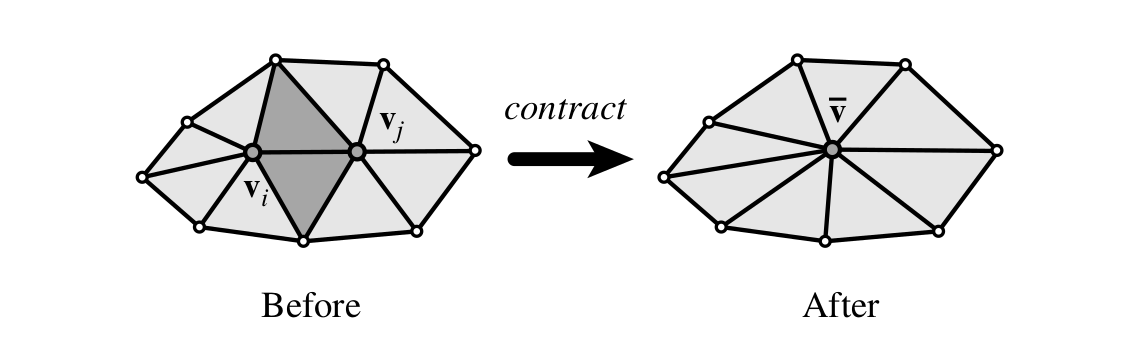
\includegraphics[width=17cm]{edge_contraction}
    \caption{Contraction of an edge \cite{garland99}.}
    \label{fig:edge_contraction_ref}
  \end{center}
\end{figure}

In the parallel framework the crucial aspect is locking all vertices and faces for the current edge to prevent from multiple threads modify the same region. To achieve this, $tryLock()$ method was used. To perform a contraction we have to check if it is possible to lock the whole neighbourhood, in the other case, it means that already a different thread is manipulating a given region. In such a situation the contraction is stopped.

The algorithm is a greedy procedure \cite{cormen01} driven by the cost of contraction. To achieve simplification we apply a sequence of edge contraction. Where the sequence is created as follows \cite{garland97}:

\begin{enumerate}
\item Select a set of candidate vertex pairs.
\item Assign a cost of contraction to each candidate.
\item Place all candidates in a heap keyed on cost with the minimum cost pair at the top.
\item Repeat until the desired approximation is reached:
\begin{enumerate}
\item Remove the pair $(\mathbf{v_i}, \mathbf{v_j})$ of least cost from the heap.
\item Contract this pair.
\item Update costs of all candidate pairs involving $\mathbf{v_i}$.
\end{enumerate}
\end{enumerate}

Each edge is associated with a cost of contraction which is basically the amount of error made during deletion of a given pair of vertices.  This cost is a key in the minimum heap \cite{cormen01} which is iteratively $pop()$. In each main iteration (steps from 1 to 4) we contract edges up to the current adaptive threshold level. If a current edge's cost is bigger or equal than the acceptable error, the main iteration procedure is stopped and the remaining egdes in the heap are ignored. In a next iteration the error is slightly increased in such a way that perviously contracted regions are even more simplified. The error calculations are based on a hyperparameter $aggressiveness$ and a current iteration value:
\begin{align}
error(i)=0.000000001*(i+3)^a
\end{align}
where $i$ is the iteration and $a$ is the aggressiveness.

\section{Assessing Cost of Contraction}
In this section I will elaborate how to measure the cost of contraction of an edge just for geometry attributes. Maintaining high level of details and faithful representation of original we should reflect the cost in the effect of changing the surface. Meaning, if the error is small the geometry changes insignificantly. An edge with a small error is a perfect candiate for removal.

Because the metric is plane-based, first, let me define a standard representation of a plane as $\mathbf{n}^T\mathbf{v}+d=0$ where $\mathbf{n} = [a\;b\;c]^T$, $d$ is a scalar constant and $\mathbf{v} = [x\;y\;z]^T$. From this, we can formulate quadric error metric as following \cite{garland99}:
\begin{align}
D^2(\mathbf{v}) = (\mathbf{n}^T\mathbf{v}+d)^2 = (ax + by + cz + d)^2
\label{quadric_distance}
\end{align}
The error for the set of planes associated with the vertex $v$ is then defiend as:
\begin{align}
\sum_{i} D_i^2(\mathbf{v}) = \sum_{i} (\mathbf{n_i}^T\mathbf{v}+d_i)^2
\end{align}
Each vertex has accumulated error metric value for surrounding faces  which represents maximum squared distance to the intersection of all planes spanned by each face.

Figure~\ref{fig:measuring_contraction_ref} shows how finding an optimal point $\bar{v}$ could look in practice in 2D. Vertices $v_i, v_j$ define set of planes $P_i = \{A,C\}$ and $P_j = \{B, C\}$. The error on each of those vertices equals $E_{plane}(v_i) = E_{plane}(v_j) = 0$ since they both lie on the lines span by thier sets. Let me define a new set which is a union of $ \bar{P} = P_i \cup P_j = \{ A,B,C \}$. Position of $\bar{v}$ minimizes the sum of square distances the the lines in $\bar{P}$ \cite{garland99}.

\begin{figure}[H]
  \begin{center}
    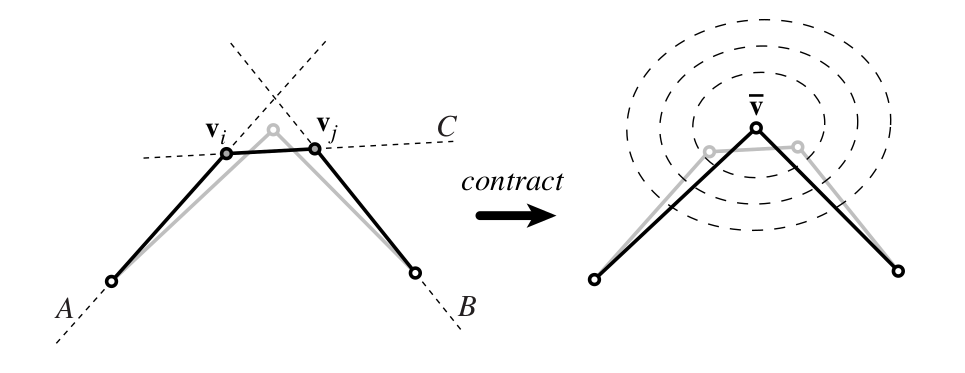
\includegraphics[width=15cm]{measuring_contraction}
    \caption{Measuring contraction cost in 2D \cite{garland99}.}
    \label{fig:measuring_contraction_ref}
  \end{center}
\end{figure}

\section{Quadric Error Metric}

In this section I will introduce the compact representation of the quadric error. First, let me expand the previously declared quadric distance $D^2(\mathbf{v})$~\ref{quadric_distance}.
\begin{align}
D^2(\mathbf{v})&=(\mathbf{n}^T\mathbf{v}+d)^2\\
	  &=(\mathbf{n}^T\mathbf{v}+d)(\mathbf{n}^T\mathbf{v}+d)\\
	  &=(\mathbf{v}^T\mathbf{n}\mathbf{n}^T\mathbf{v}+2d\mathbf{n}^T\mathbf{v}+d^2)\\
	  &=(\mathbf{v}^T(\mathbf{n}\mathbf{n}^T)\mathbf{v}+2(d\mathbf{n})^T\mathbf{v}+d^2)
	  \label{quadric_equation}
\end{align}
where $\mathbf{n}\mathbf{n}^T$ is the outer prodcut of
\begin{align}
\left[
\begin{array}{rrrr}
a^2 & ab & ac   \\
ab  & b^2 & bc  \\
ac  & bc  & c^2 \\
\end{array}\right]
\end{align}
Therefore, the $quadric\;Q$ is defined as a tripe:
\begin{align}
Q = (\mathbf{A},\mathbf{b},c)
\end{align}
Where $\mathbf{A}$ is a $3x3$ matrix, $\mathbf{b}$ is a 3-vector and c is a scalar. We can now rewrite the~\ref{quadric_equation} equation to:
\begin{align}
Q(\mathbf{v}) = \mathbf{v}^T\mathbf{A}\mathbf{v} + 2\mathbf{b}^T\mathbf{v} + c
\end{align}
Quadrics provide an intuitive addition operation which is component-wise: $Q_i(\mathbf{v}) + Q_j(\mathbf{v}) = (Q_i + Q_j)(\mathbf{v})$ where $Q_i(\mathbf{v}) + Q_j(\mathbf{v}) = (\mathbf{A_i} + \mathbf{A_j}, \mathbf{b_i} + \mathbf{b_j}, c_i + c_j)$. Using this fact we can easily define a single quadric $E_Q$ for the set of planes of a given vertex \cite{garland99} as sum over qudrics for each face:
\begin{align}
E_Q(\mathbf{v}) = \sum_{i} D_i^2(\mathbf{v}) = \sum_{i} Q_i(\mathbf{v}) = Q(\mathbf{v})
\end{align}
In other words, each vertex contains accumulated information about the error for the whole local neighbourhood of $\mathbf{v}$. For the pair of vertices the cost of contraction $(\mathbf{v_i}, \mathbf{v_j})\rightarrow\bar{\mathbf{v}}$ is simply:
\begin{align}
Q(\mathbf{\bar{v}}) = Q_i(\mathbf{\bar{v}}) + Q_j(\mathbf{\bar{v}})
\end{align}
The value of $Q(\mathbf{\bar{v}})$ is a key in the min-heap. Tables~\ref{tab:approx_bunny_ref} and~\ref{tab:wireframe_ref} show an example of simplification using quadric metric. Due to complexity of the original Stanford Bunny mesh which has 69451 faces, I first simplified it to 3642 faces and used this as a reference model.

\begin{table}[h!]
\centering
\begin{tabular}{ |c|c| } 
 \hline
 Number of faces & Original simplification\\
 \hline
 3642 faces & 94.756 \\ 
 2228 faces & 96.791 \\ 
 1842 faces & 97.347\\ 
 1152 faces & 98.341\\ 
 665 faces & 99.042\\ 
 130 faces & 99.813\\
 \hline
\end{tabular}
\caption{Percentage of simplification of the original Stanford Bunny with 69351 faces.}
\end{table}
Table~\ref{tab:original_ref} shows the quality of progressive simplification. As you can see, 70\% of reduction is hard to distinguish from the original mesh, even the 94\% is still a good approximation and features of the bunny are preserved fairly well.

\begin{center}
  	\begin{table}[H]
  	\begin{center}
  	\begin{tabular}{cc}
	\begin{subfigure}{0.7\textwidth}\centering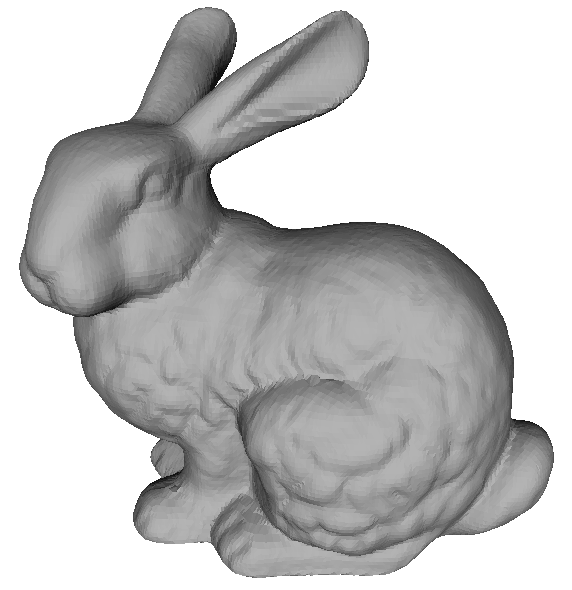
\includegraphics
		[width=0.5\columnwidth]{original_100}\caption{Faces 69451 (100\%)}\label{original_100_ref}\end{subfigure}\\
	\begin{subfigure}{0.7\textwidth}\centering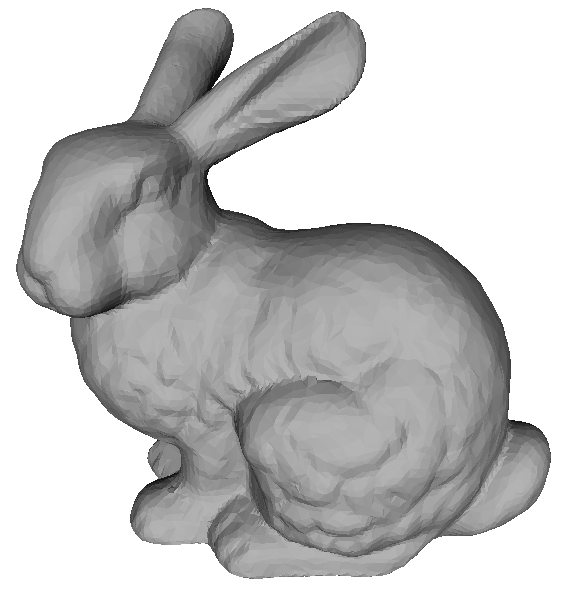
\includegraphics
		[width=0.5\columnwidth]{original_70}\caption{Faces 18892 (70\%)}\label{original_70_ref}\end{subfigure}\\
	\begin{subfigure}{0.7\textwidth}\centering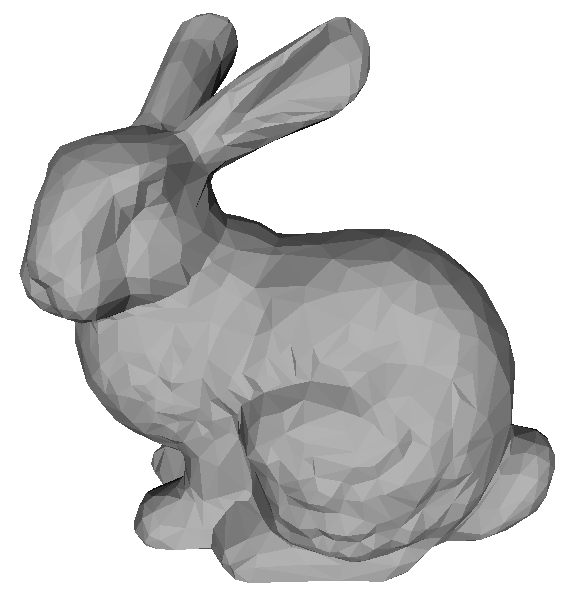
\includegraphics
		[width=0.5\columnwidth]{original_95}\caption{Faces 3642 (94\%)}\label{original_95_ref}\end{subfigure}\\
	\end{tabular}
	\caption{Quality of original mesh simplification.}
  	\label{tab:original_ref}
  	\end{center}
	\end{table}
\end{center}

\begin{center}
  	\begin{table}[H]
  	\begin{center}
  	\begin{tabular}{cc}
	\begin{subfigure}{0.4\textwidth}\centering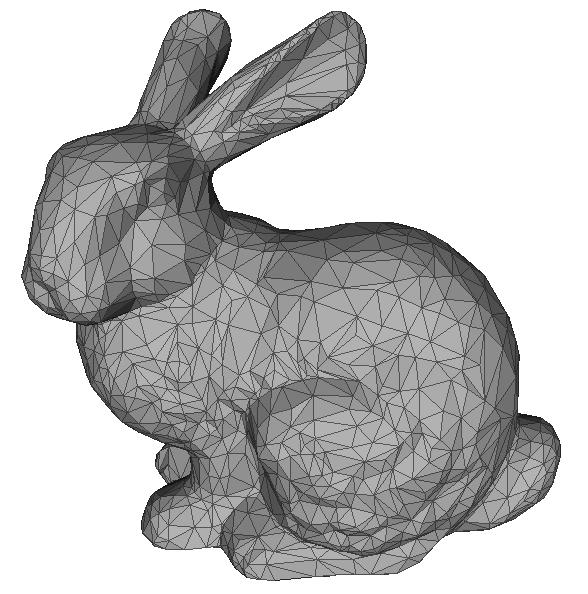
\includegraphics
		[width=0.7\columnwidth]{bunny_100}\caption{Faces 3642}\label{ref_label1}\end{subfigure}&	
	\begin{subfigure}{0.4\textwidth}\centering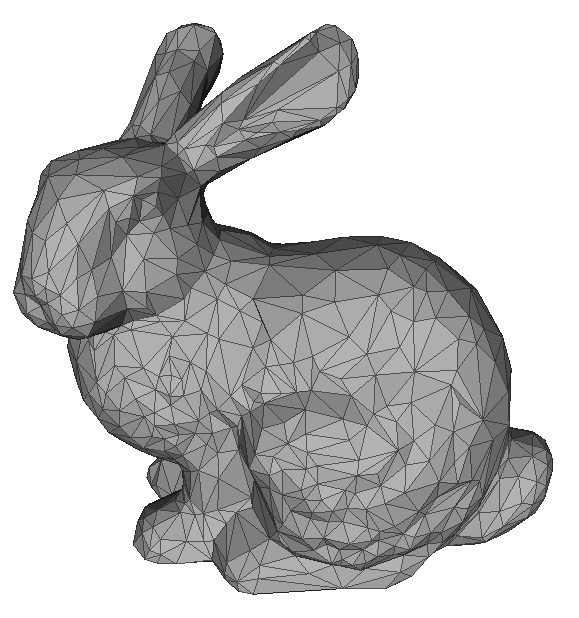
\includegraphics
		[width=0.7\columnwidth]{bunny_80}\caption{Faces 2228}\label{bunny_80_ref}\end{subfigure}\\
	\newline
	\begin{subfigure}{0.4\textwidth}\centering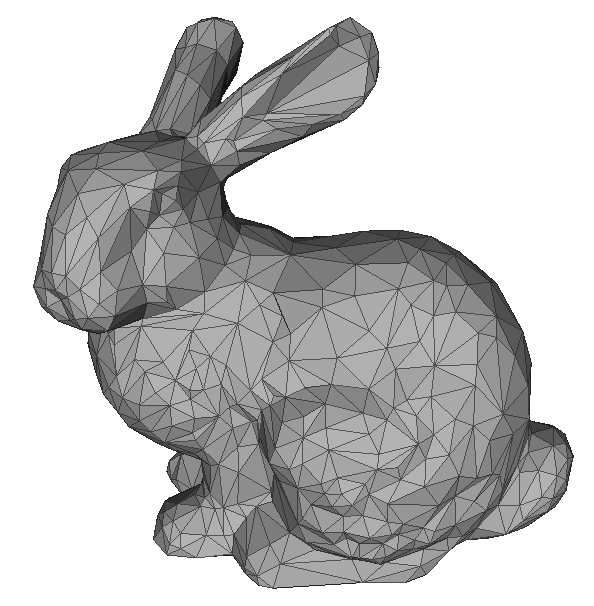
\includegraphics
		[width=0.7\columnwidth]{bunny_70}\caption{Faces 1842}\label{bunny_70_ref}\end{subfigure}&
	\begin{subfigure}{0.4\textwidth}\centering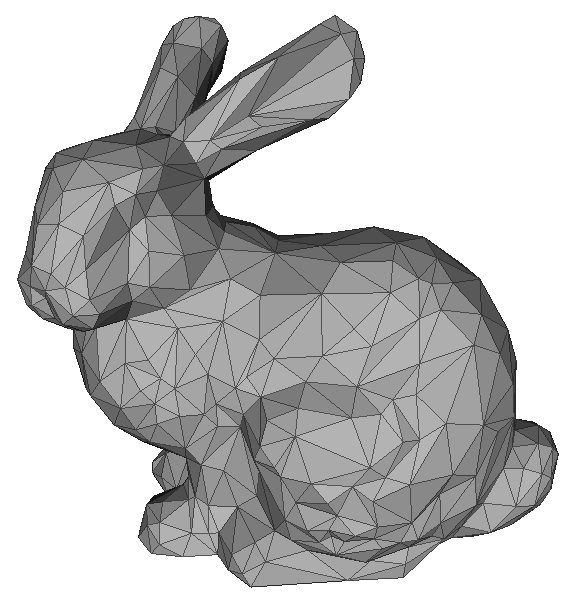
\includegraphics
		[width=0.7\columnwidth]{bunny_60}\caption{Faces 1152}\label{bunny_60_ref}\end{subfigure}\\
	\newline
	\begin{subfigure}{0.4\textwidth}\centering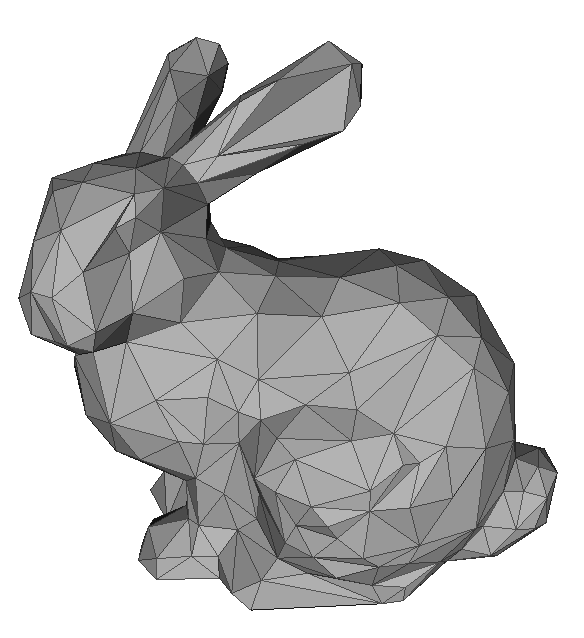
\includegraphics
		[width=0.7\columnwidth]{bunny_50}\caption{Faces 655}\label{bunny_50_ref}\end{subfigure}&
	\begin{subfigure}{0.4\textwidth}\centering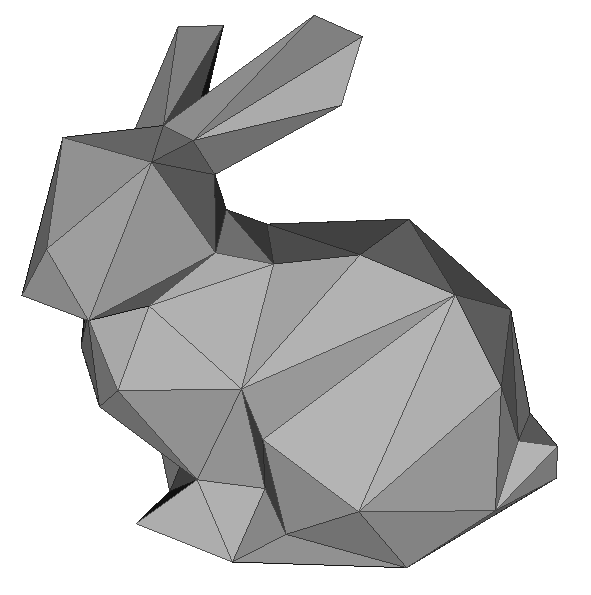
\includegraphics
		[width=0.7\columnwidth]{bunny_40}\caption{Faces 130}\label{bunny_40_ref}\end{subfigure}\\
	\end{tabular}
  	\caption{Several approximations of Stanford Bunny constructed with the geometry quadric error metric.} \label{tab:approx_bunny_ref}
  	\end{center}
	\end{table}
\end{center}

\begin{center}
  	\begin{table}[H]
  	\begin{center}
  	\begin{tabular}{cc}
	\begin{subfigure}{0.4\textwidth}\centering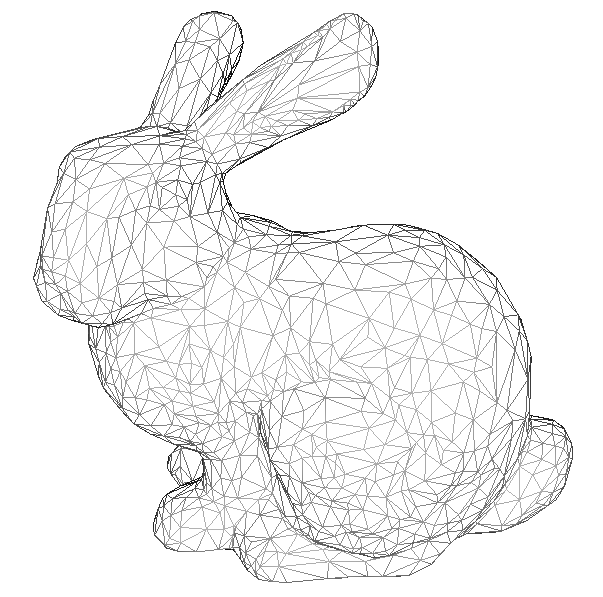
\includegraphics
		[width=0.7\columnwidth]{wireframe_100}\caption{Faces 3642}\label{wireframe_100_ref}\end{subfigure}&	
	\begin{subfigure}{0.4\textwidth}\centering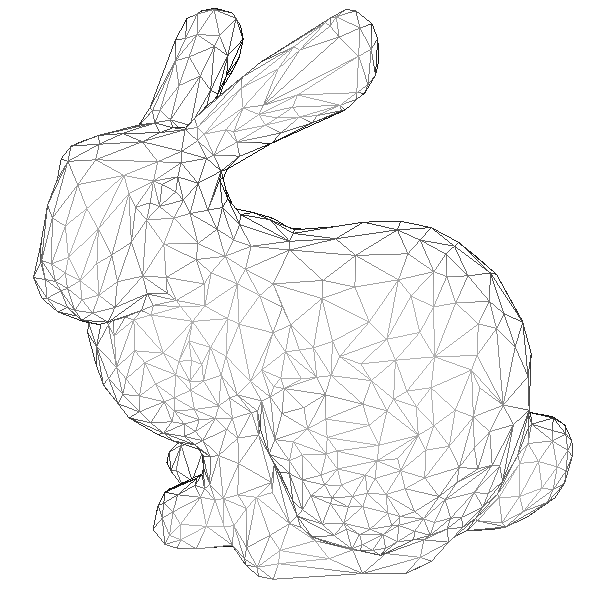
\includegraphics
		[width=0.7\columnwidth]{wireframe_80}\caption{Faces 2228}\label{wireframe_80_ref}\end{subfigure}\\
	\newline
	\begin{subfigure}{0.4\textwidth}\centering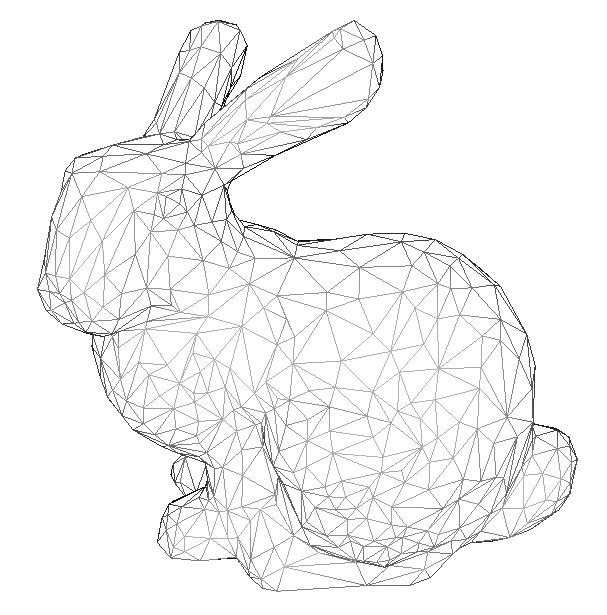
\includegraphics
		[width=0.7\columnwidth]{wireframe_70}\caption{Faces 1842}\label{wireframe_70_ref}\end{subfigure}&
	\begin{subfigure}{0.4\textwidth}\centering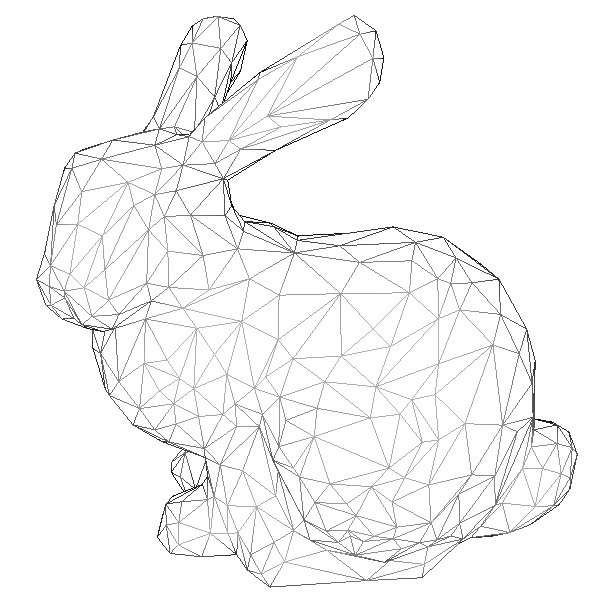
\includegraphics
		[width=0.7\columnwidth]{wireframe_60}\caption{Faces 1152}\label{wireframe_60_ref}\end{subfigure}\\
	\newline
	\begin{subfigure}{0.4\textwidth}\centering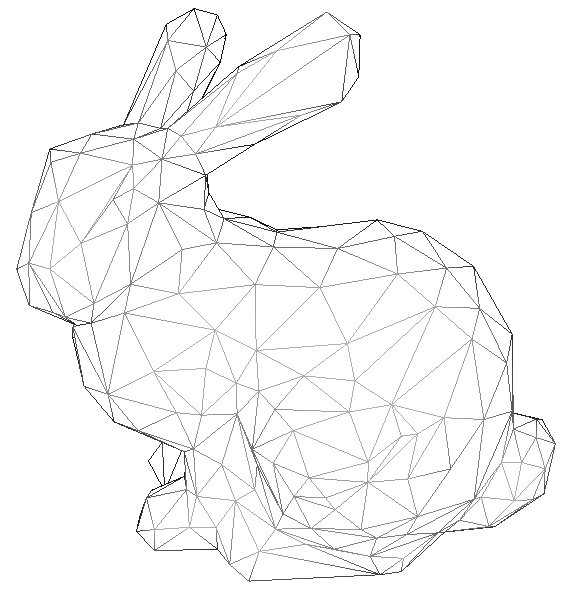
\includegraphics
		[width=0.7\columnwidth]{wireframe_50}\caption{Faces 655}\label{wireframe_50_ref}\end{subfigure}&
	\begin{subfigure}{0.4\textwidth}\centering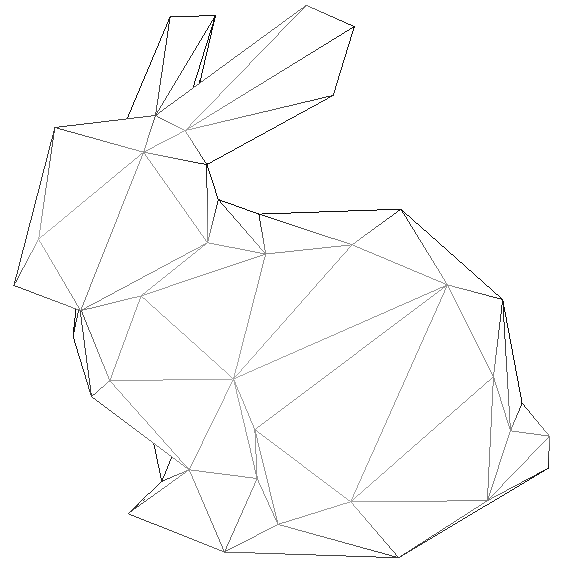
\includegraphics
		[width=0.7\columnwidth]{wireframe_40}\caption{Faces 130}\label{wireframe_40_ref}\end{subfigure}\\
	\end{tabular}
  	\caption{Wireframe versions of models in Table~\ref{tab:approx_bunny_ref}}
  	\label{tab:wireframe_ref}
  	\end{center}
	\end{table}
\end{center}

\section{Vertex Placement}

To perform the contraction of an edge $(\mathbf{v_i}, \mathbf{v_j})\rightarrow\bar{\mathbf{v}}$ we have to calcualte a new position of $\mathbf{\bar{v}}$ which is called the target. The optimal placement strategy, therefore, is to find a point for which $Q(\mathbf{\bar{v}})$ is minimal. Fortunately, since, $Q(\mathbf{\bar{v}})$ is quadratic we are guaranteed to find an unique minimizer which is a global minimum.
\begin{align}
Q(\mathbf{v}) &= \mathbf{v}^T\mathbf{A}\mathbf{v} + 2\mathbf{b}^T\mathbf{v} + c\\
\nabla Q(\mathbf{v}) &= 2\mathbf{A}\mathbf{v} + 2 \mathbf{b}
\end{align}
Solving for $\nabla Q(\mathbf{v}) = 0$, the optimal position is defined:
\begin{align}
\mathbf{\bar{v}} = -\mathbf{A}^{-1}\mathbf{b}
\end{align}
and the error:
\begin{align}
Q(\mathbf{\bar{v}}) = \mathbf{b}^T\mathbf{\bar{v}} + c = -\mathbf{b}^T\mathbf{A}^{-1}\mathbf{b} + c
\end{align}

The function used to calculate the optimal position $\mathbf{\bar{v}}$ is the following:
\begin{center}
\begin{lstlisting}[caption={LU decomposition for solving a linear system.},captionpos=b]
virtual bool optimize(Eigen::VectorXd &result) {
	Eigen::FullPivLU<Eigen::MatrixXd> lu = A.fullPivLu();
	if (!lu.isInvertible())
		return false;
	result = -lu.solve(b);
	return true;
};
\end{lstlisting}

\end{center}
Eigen::FullPivLU is LU decomposition of a matrix with complete pivoting, and related features. This decomposition provides the generic approach to solving systems of linear equations, computing the rank, invertibility, inverse, kernel, and determinant \cite{eigenLU19}.
\chapter{Extended simplification algorithm}
\thispagestyle{empty}% no page number in chapter title page
\section{Design}
